\section{La formation}

\subsection{Contenu}

La formation dispensée a pour but principal de mettre tous les stagiaires au même niveau sur les principales technologies Java/JEE utilisées dans le monde de l'entreprise.\\

Nous avons ainsi abordé les sujets suivants :

\begin{itemize}
	\item eXtreme Programming
	\item UML
	\item Subversion
	\item Maven 2
	\item Java 5
	\item Log4J
	\item JDBC
	\item JUnit 3 et 4
	\item JEE
	\item Hibernate 3
	\item Spring 2.5\\
\end{itemize}

Les technologies abordées sont pour la plupart survolées et certaines sont dépassées, bien que toujours grandement utilisées. La formation sert ainsi de socle pour une auto-formation plus en détail de ces même technologies ou bien de leurs successeurs. Cette auto-formation est une composante indispensable du métier de consultant puisqu'elle permet de rester à un certain niveau d'expertise, de pouvoir anticiper les évolutions techniques et, éventuellement, de pouvoir être force de proposition sur la direction d'un projet.

\subsection{Déroulement}

L'ensemble de la formation se fait via la plateforme d'e-learning développée par \excilys{}, à savoir Capico \cite{capico}. Elle consiste en une suite de cours magistraux éventuellement sonorisés pour une meilleure compréhension. Ces cours sont accompagnés de QCM pour vérifier que les connaissances ont bien été assimilées ainsi que d'exercices pour la mise en pratique.

\begin{figure}[H]
	\centering
	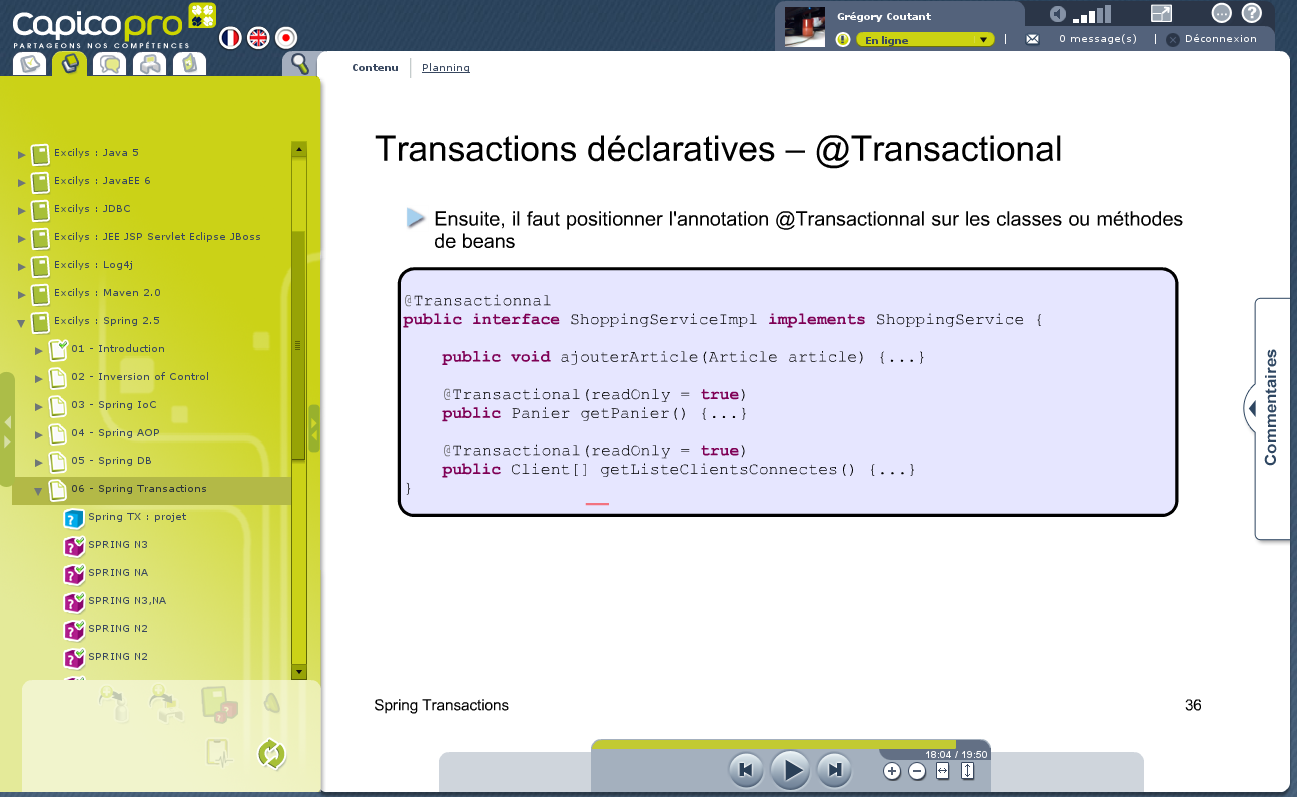
\includegraphics[width=\linewidth]{images/capico.pdf}
	\caption{Éxemple de cours sur Capico}
\end{figure}

Stéphane LANDELLE est responsable de la formation des stagiaires. Il s'assure donc du bon suivi de la formation et la ponctue d'interventions visant à vérifier nos connaissances ou à éclaircir certains points qui pourraient être compliqués. Il permet aussi d'apporter un point de vue plus pratique sur ces technologies, notamment comment elles sont utilisées dans le monde de l'entreprise ou comment elles devraient l'être.

\subsection{Technologies abordées}

Les technologies abordées lors de la formation étant en partie utilisées pendant le reste du stage, je vais maintenant les présenter brièvement pour une meilleure compréhension de la suite du rapport.

\subsubsection{eXtreme Programming (XP)}

XP est une méthode Agile utilisée dans le développement logiciel assez proche d'une autre méthode Agile plus connue : la méthode Scrum \cite{scrum}. Elle découpe le développement d'une application en plusieurs sprints d'une à deux semaines. Le développement est ainsi incrémental garantissant la sortie d'une application fonctionnelle à chaque fin de sprint. Le développement incrémental permet d'avoir un développement plus souple.\\

XP s'appuie notamment sur le pair programming qui consiste à travailler en binôme sur un même ordinateur avec un \emph{pilote} qui contrôle le clavier et la souris et un \emph{copilote} qui a plus de recul et aide le \emph{pilote}. Régulièrement, les rôles s'inversent.\\

Un autre principe de cette méthode est le Test Driven Development (TDD). TDD vise à rendre le développement plus simple et efficace en écrivant d'abord les tests permettant de garantir qu'une fonctionnalité a été développée puis en développant la fonctionnalité. L'idée est de simplement écrire le code qui garantit que les tests passent. Cette méthodologie vise à écrire du code de qualité et fonctionnellement correct, et à faciliter la maintenance de celui-ci. 

\subsubsection{Maven}

Maven \cite{maven} est un outil de gestion et de construction de projets Java. Une de ses forces est notamment de gérer les librairies externes ou bien la sortie d'une nouvelle version. Maven permet d'automatiser la plupart des tâches liées à un projet informatique : récupération des librairies externes, compilation, exécution des tests, génération des livrables, déploiement de l'application sur un serveur, \dots Ce type d'outil est quasiment indispensable pour un projet Java. Maven est la solution la plus utilisé mais d'autres alternatives existe comme Ant ou Gradle. 

\subsubsection{Java}

Java \cite{java} est un langage de programmation orienté objet développé par Sun Microsystems (racheté par Oracle Corporation). Il est vraisemblablement le langage les plus utilisé en entreprise. C'est un langage compilé qui s'exécute sur une machine virtuelle appelée Java Virtual Machine (JVM), ce qui permet aux applications Java d'être portables puisque seule la JVM dépend du système d'exploitation.\\

Un des principes fondamentaux de Java qui fait de lui un langage très apprécié des entreprise est la garantie de la rétro-compatibilité entre différentes versions de Java. Ainsi une application développée en Java 1.4 peut fonctionner sur une JVM Java 7, profitant ainsi des améliorations apportées à celle-ci.

\subsubsection{JUnit}

JUnit \cite{junit} est un framework permettant d'effectuer facilement des tests unitaires. C'est actuellement le framework le plus utilisé pour les tests dans le monde Java ce qui lui permet d'être très bien intégré dans les environnements de développement tels qu'Eclipse, ou dans des outils comme Maven.

\subsubsection{Java Enterprise Edition (JEE)}

JEE \cite{jee} est une plateforme de développement d'applications d'entreprise décrite par un ensemble de spécifications (28 spécifications pour JEE 6) appelées JSR permettant de normaliser les technologies utilisées telles que :

\begin{description}
	\item[Servlets] objets Java capable de répondre à des requêtes HTTP,
	\item[Java Server Pages (JSP)] langage permettant de générer dynamiquement des pages HTML en s'interfaçant facilement avec du code Java,
	\item[Java Persistence API (JPA)] API inspirée d'Hibernate, permettant de rendre persistant dans une base de données relationnelles des objets Java,
	\item[Entreprise JavaBean (EJB)] architecture coté serveur servant à créer des composants distribués.
\end{description}

\subsubsection{Java DataBase Connectivity (JDBC)}

JDBC \cite{jdbc} est une API permettant la communication avec des bases de données relationnelles. JDBC permet de s'abstraire du langage de requêtes utilisé par la base de données. La traduction des requêtes se fait en temps réel par le pilote spécifique à la base de données utilisée.

\subsubsection{Hibernate}

Hibernate \cite{hibernate} est un framework d'Object Relational Mapping (ORM), c'est à dire un framework permettant de faire la passerelle entre une représentation objet d'un modèle et sa représentation relationnelle. Il permet ainsi de persister de façon simple et intuitive les objets Java dans une base de données relationnelle. Hibernate s'occupe de faire le lien entre les classes et attributs Java et les tables d'une base de données. Depuis sa version 4, Hibernate est une des implémentation de JPA.

\subsubsection{Spring}

Le framework Spring \cite{spring} est une alternative et un concurrent à la plateforme JEE. L'idée est de proposer au développeur un ensemble de fonctionnalités à la manière de JEE mais sous la forme de dépendances modulaires. Ainsi, une application Spring peut fonctionner sur une simple JVM ou sur un serveur léger tel que Tomcat ou Jetty. Au contraire d'une application JEE qui se déploie uniquement dans un conteneur lourd, ou serveur d'application, tel que Glassfish ou JBoss implémentant toutes les JSR de la spécification JEE. Les applications JEE sont extrêmement dépendantes du conteneur ce qui restreint la portabilité de l'application, à la différence d'une application Spring.\\

Le c\oe{}ur de Spring est une implémentation du design pattern Inversion of Control (IoC) : l'instanciation des classes n'est plus à la charge du développeur mais du framework. Ceci permet ainsi de l'injection de dépendance, c'est à dire, d'automatiquement injecter à l'exécution les dépendances d'un objet lors de son instanciation. On peut donc modifier le comportement de l'application à l'exécution. Tous les modules de Spring reposent sur cette fonctionnalité. La déclaration des instances gérées par Spring se fait via un fichier XML ou via des annotations directement dans le code. On peut donc voir Spring comme une fabrique d'objets (design pattern Factory).\\

De nombreux modules font de Spring une énorme boite à outils : intégration avec un ORM (Hibernate, JPA, \dots), programmation orientée aspect (AOP), implémentation du design pattern MVC pour faciliter la création d'application web, intégration dans les frameworks de tests unitaires (JUnit), \dots

\subsection{Formation continue}

Après la phase de formation du stage terminée, j'ai, parallèlement au travail demandé, continué et approfondi plusieurs sujets pour ma curiosité personnelle mais aussi parce que c'est un des devoirs d'un consultant du \excilysGroup{}.\\

En premier lieu, j'ai approfondi mes connaissances en Java pur pour notamment pouvoir passer l'examen d'Oracle Certified Java SE 6 Programmer (OCJP). Cet examen permet d'être certifié par Oracle comme \flqq{}maîtrisant le langage Java\frqq{} si le score obtenu est supérieur à 61 \%. Cette certification est nécessaire pour être embauché dans le \excilysGroup{}. J'ai obtenu la note de 91 \%.\\

En second lieu, je me suis aussi intéressé à des technologies émergentes comme Scala, Play! 2 ou bien Gradle.